\documentclass[hidelinks]{article}
\usepackage[spanish]{babel}
\usepackage{amsmath}
\usepackage{hyperref}
\newcommand\Omicron{O}
\usepackage{graphicx}
\newcommand{\br}{\vskip.2cm \noindent}
\usepackage{verbatim}

\graphicspath{ {./} }


\newtheorem{respuesta}{Respuesta}

\author{Santiago Sinisterra Sierra}
\title{Diseño y Análisis de Algoritmos \\ Examen 1}
\date{\today}

\begin{document}

\maketitle

\section{Problema 1}

Para que $f(n)$ sea $\Theta(n^3)$ es necesario encontrar dos constantes $c_1$ y $c_2$ así como un valor $n_0$ que haga que  la Ec.(\ref{eq:prob01_propiedad}) se cumpla.

\begin{equation}
  \label{eq:prob01_propiedad}
  c_1 n^3 \leq f(n) \leq c_2 n^3
\end{equation}

En primera instancia se desarrolla $f(n)$, el cual se muestra en la Ec.(\ref{eq:prob01})

\begin{equation}
  \label{eq:prob01}
  \begin{aligned}
    f(n) & = 32n ( \frac{n-1}{2} + 3) + 8n^2 + 10n + 4     \\
    f(n) & = 32n ( \frac{n^2 - n + 6}{2}) + 8n^2 + 10n + 4 \\
    f(n) & = 16n ( n^2 - n + 6) + 8n^2 + 10n + 4           \\
    f(n) & = 16n^3 - 16n^2 + 96n + 8n^2 + 10n + 4          \\
    f(n) & = 16n^3 - 8n^2 + 106n + 4                       \\
  \end{aligned}
\end{equation}

En la Ec.(\ref{eq:prob01a}) se calcula $c_1$, resolviendo la desigualdad de la primera línea.

\begin{equation}
  \label{eq:prob01a}
  \begin{aligned}
    c_1 n^3                    & \leq 16n^3 - 8n^2 + 106n + 4                             \\
    c_1 n^3 - 16n^3            & \leq -8n^2 + 106n + 4                                    \\
    (c_1 - 16) n^3             & \leq -8n^2 + 106n + 4                                    \\
    \frac{(c_1 - 16) n^3}{n^3} & \leq \frac{ -8n^2 + 106n + 4        }{n^3}               \\
    (c_1 - 16 )                & \leq \frac{-8}{n} + \frac{106}{n^2} + \frac{4}{n^3}      \\
    (c_1 - 16 )                & \leq \frac{-8}{n} + \frac{106}{n^2} + \frac{4}{n^3}      \\
    c_1                        & \leq \frac{-8}{n} + \frac{106}{n^2} + \frac{4}{n^3} + 16
  \end{aligned}
\end{equation}

En la Ec.(\ref{eq:prob01b}) se calcula $c_2$, resolviendo la desigualdad de la primera línea.

\begin{equation}
  \label{eq:prob01b}
  \begin{aligned}
    c_2 n^3                    & \geq 16n^3 - 8n^2 + 106n + 4                             \\
    c_2 n^3 - 16n^3            & \geq -8n^2 + 106n + 4                                    \\
    (c_2 - 16) n^3             & \geq -8n^2 + 106n + 4                                    \\
    \frac{(c_2 - 16) n^3}{n^3} & \geq \frac{ -8n^2 + 106n + 4        }{n^3}               \\
    (c_2 - 16 )                & \geq \frac{-8}{n} + \frac{106}{n^2} + \frac{4}{n^3}      \\
    (c_2 - 16 )                & \geq \frac{-8}{n} + \frac{106}{n^2} + \frac{4}{n^3}      \\
    c_2                        & \geq \frac{-8}{n} + \frac{106}{n^2} + \frac{4}{n^3} + 16
  \end{aligned}
\end{equation}

Evaluando la Ec.(\ref{eq:prob01a})con $n = n_0$ con un $n_0$ seleccionado de $20$ para obtener $c_1$

\begin{equation}
  \label{eq:prob01c}
  \begin{aligned}
    c_1 & \leq \frac{-8}{n} + \frac{106}{n^2} + \frac{4}{n^3} + 16 \\
    c_1 & \leq \frac{-8}{20} + \frac{106}{20^2} + \frac{4}
    {20^3} + 16                                                    \\
    c_1 & \leq \frac{31731}{2000}
  \end{aligned}
\end{equation}

\br Evaluando la Ec.(\ref{eq:prob01d}) con $n = n_0$ con un $n_0$ seleccionado de $20$ para obtener $c_2$

\begin{equation}
  \label{eq:prob01d}
  \begin{aligned}
    c_2 & \geq \frac{-8}{n} + \frac{106}{n^2} + \frac{4}{n^3} + 16 \\
    c_2 & \geq \frac{-8}{20} + \frac{106}{20^2} + \frac{4}
    {20^3} + 16                                                    \\
    c_2 & \geq \frac{31731}{2000}
  \end{aligned}
\end{equation}

\br Con un $c_1$ y $c_2$ calculado, se sustituye la propiedad inicial en la Ec.(\ref{eq:prob01_propiedad}), resultando en la Ec.(\ref{eq:prob01_dem})

\begin{equation}
  \label{eq:prob01_dem}
  \begin{aligned}
    c_1 n^3 \leq                   & f(n) \leq c_2 n^3                 \\
    \frac{31731}{2000} (20)^3 \leq & f(20) \leq \frac{31731}{2000} n^3 \\
    126924 \leq                    & 126924
    \leq 126924
  \end{aligned}
\end{equation}

\br Al realizar la evaluación de la Ec.(\ref{eq:prob01_dem}) y verificarse que se cumple la propiedad, se completa la demostración.

\section{Problema 2}
\br Sólo hay un orden topológico: a, c, b, d.

\br Siempre se inicia por $a$ porque es el único nodo sin aristas que entran. $b$ no puede ser el segundo elemento porque no hay forma de eliminar la arista $(c,b)$ sin antes agregar al orden a $c$; por lo que $c$ es el segundo elemento y $c$ el tercero. $d$ tiene que ser el último elemento porque no sale ninguna arista del mismo.

\section{Problema 3}
\subsection{(a)}
\br $O(f(n))$ es $n^3$, ya que primero hay que recorrer $i$ de $1$ a $n$. Para cada elemento en $i$, hay que recorrer $j$ hasta $n$. Finalmente, para $B_{ij}$ hay que sumar en un rango, el cual es una operación a la que le toma $n$ pasos. Multiplicando, resulta en $n \cdot n \cdot n = n^3$. Ya que es posible encontrar una $c$ (1) y $n_0$ (1) tal que $c g(n) \geq f(n)$, $f(n)$ forma parte de $O$.

\subsection{(b)}

\br Para que $f(n)$ sea $\Omega(n^3)$ se debe encontrar una $c$ (1) y $n_0$ (1) tal que $c g(n) \leq f(n)$, $f(n)$ forma parte de $\Omega$.

\br Como previamente se comprobó que $f(n)$ es tanto $O(n^3)$ como $\Omega(n^3)$; $f(n)$ pertenece a $\Theta(n^3)$ ya que la condición es que debe pertenecer tanto a $O$ como a $\Omega$.

\subsection{(c)}
\br En lugar de sumar de $A_i$ hasta $A_j$, se reemplaza la línea 3 del algoritmo 1 por $B_{i, j} <- B{i, j-1} + A_j$. Se elimina la $n$ extra porque la suma y el acceso tienen costo constante. El pseudocódigo queda en la Fig.(\ref{fig:codigo})

\begin{figure}[h!]
  \begin{verbatim}
    for i = 1, 2, ..., n do
      for j = i + 1, i + 2, ..., n do
          Bij <- B[i, j-1] + A[j]
      end
    end
  \end{verbatim}
  \label{fig:codigo}
  \caption{Fig(3.3.)}
\end{figure}

\br Este algoritmo pertenece a $O(n^2)$, al calcular el límite se divide $\frac{n^2 }{n^2} = 1$ , donde su límite es 0.

\section{Problema 4}

\br Para determinar si un grafo no contiene ciclos se puede recorrer el grafo con el algoritmo de búsqueda en profundidad (DFS). Se puede plantear como una versión modificada de DFS, cuando $v$ es un nodo ya marcado entonces significa que ya fue visitado previamente, generando un ciclo. Si se encuentra un ciclo, se activa una bandera en el procedimiento que marca que se encontró un ciclo. Si el algoritmo no tiene ciclos, regresa verdadero si $ciclo\_detectado$ es falso. En la Fig.(\ref{fig:algoritmo2}) está el pseudocódigo del algoritmo

\begin{figure}
  \begin{verbatim}
    ciclo_detectado <- false
    explorados <- [(n, false) for n in nodos(G)]

    def DFS(G, u):
      marcar la arista u como explorada
      foreach Arista(u,v) do:
        if not marcado(v):
          DFS(G, v)
        else
          ciclo_detectado <- true
        end
      end
    return ciclo_detectado == false
  \end{verbatim}
  \caption{Algoritmo para el problema 4}
  \label{fig:algoritmo2}
\end{figure}

\br Tiene complejidad $O(m + n)$ porque la iteración del foreach lo hace para m aristas, y la inicialización de la lista de explorados lo hace para n nodos.

\section{Problema 5}
\subsection{(a)}
El árbol de expansión mínima está dado en la Fig.(\ref{fig:diagrama})

\begin{figure}[h]
  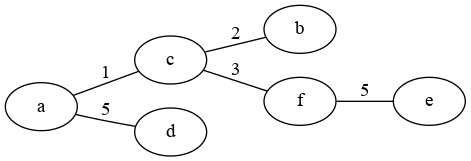
\includegraphics[width=\textwidth]{diagrama.png}
  \caption{MST propuesto}
  \label{fig:diagrama}
\end{figure}

\begin{enumerate}
  \item Se selecciona de la cola de prioridad la arista de menor peso (a,c) y se comprueba que no forme ciclos en el árbol
  \item La siguiente de menor peso es (b,c). Como no forma ciclos en el árbol, se agrega al árbol.
  \item La siguiente de menos peso es (c, f). Como no forma ciclos, se agrega al árbol
  \item La siguiente de menor peso es (a, b). Pero al agregarla se forma un ciclo (a, b, c), por lo cual se descarta.
  \item La siguiente de menor peso es (a, d). Como no forma ciclos en el árbol, se agrega al árbol
  \item La siguiente de menor peso es (f, e). Como no forma ciclos en el árbol, se agrega al árbol.
  \item La siguiente de menor peso es (d, f). Si se agregara, formaría un ciclo entre ACDF, por lo cual se descarta.
  \item Finalmente está (a, e). Si se agregara, forma un ciclo entre ACFE, por lo que se descarta
\end{enumerate}

\br Una vez evaluados todas las aristas, el algoritmo termina.

\subsection{(b)}
\br (d,f) no puede formar parte de ningún MST porque el algoritmo nunca la consideraría al ser un algoritmo voraz. Los vértices que conecta siempre tienen una opción mejor para unirse al árbol que (d,f), que se evalúan antes porque las aristas siempre se mantienen ordenadas.

\br Para uno de los vértices que conecta, d, siempre se evalúa antes (a, d) ya que tiene menor costo que (d, f). Del mismo modo, para que f se conecte con otros nodos, (c,f) y (f,e) siempre se evalúan antes de (d,f), los cuales tienen costo menor que (d,f).

\end{document}